\documentclass[11pt,a4paper]{article}

% -----------------------------------------------------------------------------
% PACKAGES & CONFIGURATION
% -----------------------------------------------------------------------------
\usepackage[utf8]{inputenc}
\usepackage[T1]{fontenc}
\usepackage{lmodern}
\usepackage{microtype}
\usepackage[margin=1.8cm,top=2.0cm,bottom=2.0cm,headheight=14pt]{geometry}
\usepackage{graphicx}
\usepackage{xcolor}
\usepackage{fancyhdr}
\usepackage{titlesec}
\usepackage{amsmath,amssymb}
\usepackage{booktabs}
\usepackage{array}
\usepackage{caption}
\usepackage{float}
\usepackage{subcaption}
\usepackage{needspace}
\usepackage{tcolorbox}
\tcbuselibrary{skins,listings}
\usepackage{hyperref}

% -----------------------------------------------------------------------------
% COLOR DEFINITIONS (ENSIA Lab Theme)
% -----------------------------------------------------------------------------
\definecolor{primary}{RGB}{31, 78, 121}        % Deep Navy Blue (#1f4e79)
\definecolor{darktext}{RGB}{30, 30, 30}        % Text color
\definecolor{codebg}{RGB}{246, 247, 249}       % Shaded code box background
\definecolor{codeborder}{RGB}{195, 205, 215}   % Code box border
\definecolor{barcolor}{RGB}{31, 78, 121}       % Left accent bar

% -----------------------------------------------------------------------------
% GRAPHICS PATH
% -----------------------------------------------------------------------------
\graphicspath{{screenshots/}{plots/}}

% -----------------------------------------------------------------------------
% HEADERS & FOOTERS (Matching ENSIA Lab Sheet)
% -----------------------------------------------------------------------------
\pagestyle{fancy}
\fancyhf{}
\fancyhead[L]{\small\textit{ENSIA -- AI and Data Science}}
\fancyhead[R]{\small\textit{Introduction to Mobile Robotics}}
\fancyfoot[L]{\small\textit{Lab 3: Pose Control of a Differential Drive Robot -- Solution Report}}
\fancyfoot[R]{\small\textit{Page \thepage}}
\renewcommand{\headrulewidth}{0.5pt}
\renewcommand{\footrulewidth}{0.5pt}

% -----------------------------------------------------------------------------
% SECTION TITLE FORMATTING
% -----------------------------------------------------------------------------
\titleformat{\section}
  {\color{primary}\Large\bfseries}{\thesection.}{0.6em}{}

\titleformat{\subsection}
  {\color{primary}\large\bfseries}{}{0pt}{}

\titleformat{\subsubsection}
  {\color{primary}\normalsize\bfseries}{}{0pt}{}

\titlespacing*{\section}{0pt}{10pt plus 1pt minus 1pt}{5pt}
\titlespacing*{\subsection}{0pt}{8pt plus 1pt minus 1pt}{4pt}
\titlespacing*{\subsubsection}{0pt}{6pt plus 1pt minus 1pt}{3pt}

% -----------------------------------------------------------------------------
% COMMAND & CODE LISTING STYLING
% -----------------------------------------------------------------------------
\lstset{
  basicstyle=\footnotesize\ttfamily,
  backgroundcolor=\color{codebg},
  frame=leftline,
  framerule=2.5pt,
  rulecolor=\color{barcolor},
  breaklines=true,
  columns=fullflexible,
  keepspaces=true,
  showstringspaces=false,
  xleftmargin=3mm,
  aboveskip=6pt,
  belowskip=6pt
}

\captionsetup{
  font=small,
  labelfont={bf,color=primary},
  labelsep=period,
  skip=4pt
}

\hypersetup{
  colorlinks=true,
  linkcolor=primary,
  citecolor=primary,
  urlcolor=primary,
  pdfauthor={BELHIMER Mohamed Ayoub},
  pdftitle={LAB 3 REPORT - BELHIMER Mohamed Ayoub - Group 1}
}

% -----------------------------------------------------------------------------
% DOCUMENT BODY
% -----------------------------------------------------------------------------
\begin{document}

% -----------------------------------------------------------------------------
% DIRECT SOLUTION HEADER
% -----------------------------------------------------------------------------
\begin{center}
  {\LARGE \textbf{\color{primary}LAB 3 REPORT}}\\[0.25cm]
  {\large \textbf{BELHIMER Mohamed Ayoub} \quad \textbullet \quad \textbf{Group 1}}\\[0.25cm]
  \rule{\linewidth}{0.8pt}
\end{center}
\vspace{-0.1cm}

% =============================================================================
% SECTION 1: STATE FEEDBACK CONTROL
% =============================================================================
\section{State Feedback Control}
\subsection*{Tasks}

\subsubsection*{Task 1: CoppeliaSim Scene Initialization (\texttt{ENSIA\_IMR\_Lab3.ttt})}
CoppeliaSim was launched and the laboratory scene \texttt{ENSIA\_IMR\_Lab3.ttt} was loaded. The Pioneer P3-DX differential-drive robot starts near the world origin $(x_0, y_0, \theta_0) \approx (0, 0, 0)$ and interfaces with ROS 2 through the \texttt{/pose} (\texttt{geometry\_msgs/msg/Pose2D}) and \texttt{/cmd\_vel} (\texttt{geometry\_msgs/msg/Twist}) topics.

\begin{figure}[H]
  \centering
  \begin{subfigure}[b]{0.49\linewidth}
    \centering
    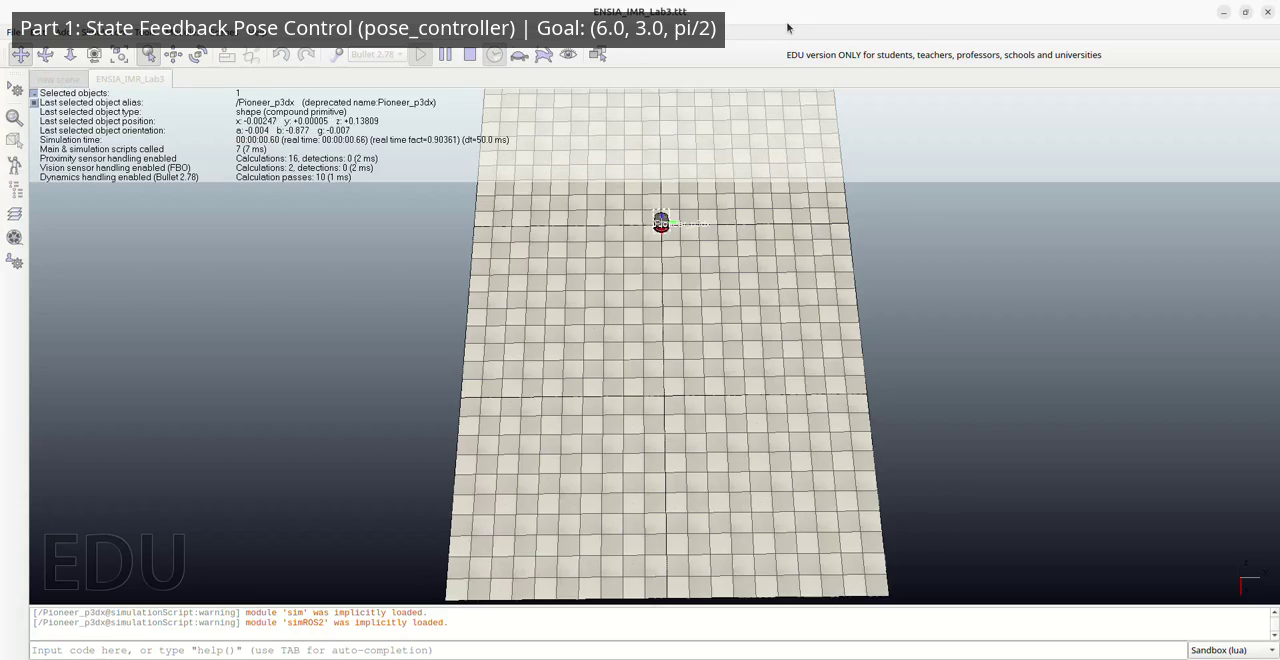
\includegraphics[width=\linewidth]{sim_p1_start.png}
  \end{subfigure}
  \hfill
  \begin{subfigure}[b]{0.49\linewidth}
    \centering
    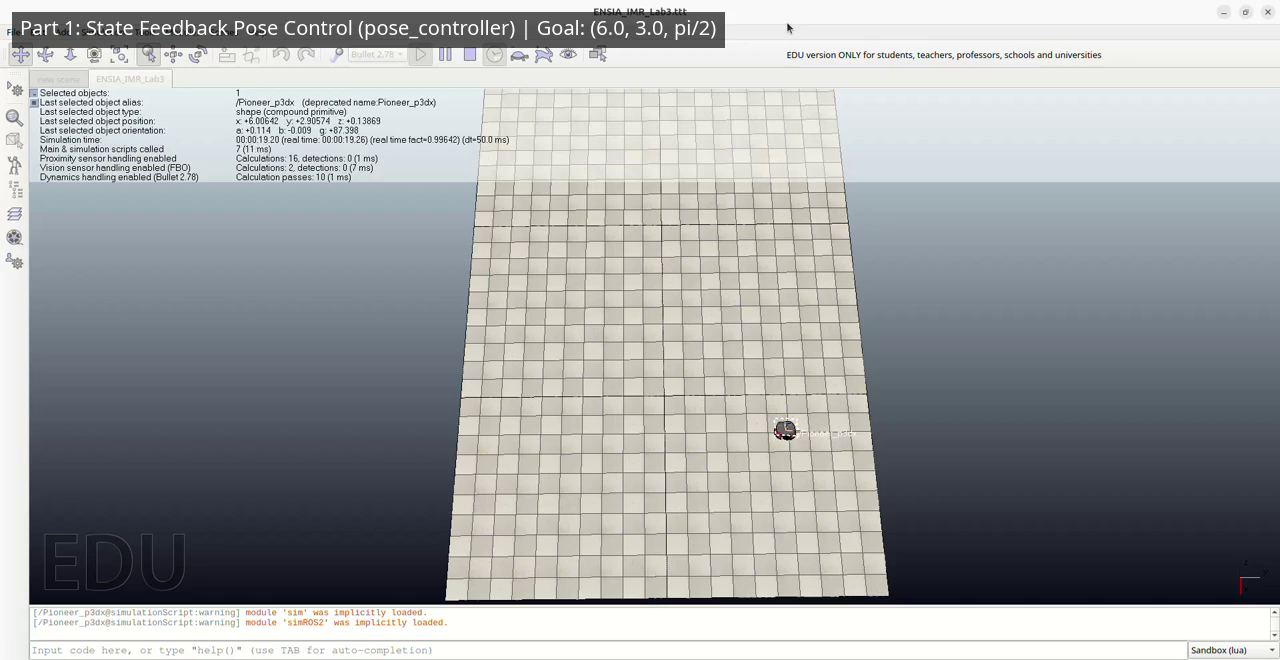
\includegraphics[width=\linewidth]{sim_p1_goal.png}
  \end{subfigure}
  \caption{CoppeliaSim scene \texttt{ENSIA\_IMR\_Lab3.ttt}: initial robot pose near $(0, 0, 0)$ (left) and converged final pose near $(6.0, 3.0, \pi/2)$ under \texttt{pose\_controller} (right).}
  \label{fig:sim_p1}
\end{figure}

\subsubsection*{Tasks 2--4: ROS 2 Package and Node Setup}
A ROS 2 Python package named \texttt{pionner\_p3dX\_controller} was created inside \texttt{\textasciitilde/ros2\_ws/src/}. The controller node \texttt{pose\_controller} was implemented in \texttt{pionner\_p3dX\_pose\_controller.py}, with:
\begin{itemize}
  \item A subscriber on \texttt{/pose} (\texttt{geometry\_msgs/msg/Pose2D}) bound to \texttt{self.pose\_callback}.
  \item A publisher on \texttt{/cmd\_vel} (\texttt{geometry\_msgs/msg/Twist}) sending computed $(v, \omega)$ commands.
\end{itemize}

\subsubsection*{Task 5: Role of Callback Functions and \texttt{rclpy.spin()} / \texttt{rclcpp::spin()}}
In a ROS 2 node, incoming topic data is processed asynchronously via an event-driven architecture:
\begin{itemize}
  \item \textbf{Callback Function (\texttt{pose\_callback} / \texttt{poseCallback}):} Defines the reaction executed whenever a new message arrives on the subscribed topic (\texttt{/pose}). In this controller, it extracts the robot's current pose $(x, y, \theta)$, transforms Cartesian errors into polar goal coordinates $(\rho, \alpha, \beta)$, evaluates the state-feedback control law, and publishes the resulting velocity command to \texttt{/cmd\_vel}.
  \item \textbf{\texttt{rclpy.spin(node)} / \texttt{rclcpp::spin(node)}:} Runs the ROS 2 executor's blocking event loop. It keeps the node alive, continuously polls DDS middleware queues for incoming messages, timers, and service requests, and dispatches each received \texttt{/pose} message to \texttt{pose\_callback} until shutdown (\texttt{Ctrl+C}).
  \item \textbf{Interaction:} \texttt{spin()} acts as the scheduler and dispatcher, while the callback supplies the user logic. Every simulator pose update wakes up \texttt{spin()}, which invokes \texttt{pose\_callback}, closing the feedback control loop at the simulator's publishing rate ($20\,\text{Hz}$, $\Delta t = 50\,\text{ms}$) without busy-waiting.
\end{itemize}

\subsubsection*{Task 6: Closed-Loop Controller Implementation, Gain Tuning, and Build}
Using the relative polar coordinates $(\rho, \alpha, \beta)^T$:
\begin{align}
  \rho &= \sqrt{(x_g - x)^2 + (y_g - y)^2}, &
  \phi &= \operatorname{atan2}(y_g - y,\, x_g - x), \\
  \alpha &= \operatorname{wrap}(\phi - \theta), &
  \beta &= \operatorname{wrap}(\theta_g - \phi),
\end{align}
the state-feedback control law (Equations 1 and 2) was implemented as:
\begin{equation}
  v = k_\rho \rho, \qquad \omega = k_\alpha \alpha + k_\beta \beta,
\end{equation}
with velocity saturation $v \in [0, v_{\max}]$ ($v_{\max} = 0.6\,\text{m/s}$) and $\omega \in [-\omega_{\max}, \omega_{\max}]$ ($\omega_{\max} = 1.2\,\text{rad/s}$). Once the robot enters the position tolerance ($\rho \le 0.1\,\text{m}$), linear motion stops ($v = 0$) and proportional rotation ($\omega = \Delta\theta$) aligns $\theta$ within $|\Delta\theta| \le 0.05\,\text{rad}$.

\paragraph{Parameter Configuration and Stability Verification:}
All parameters for the goal $(x_g, y_g, \theta_g) = (6.0,\, 3.0,\, \pi/2)$ and gains $k_\rho = 0.5$, $k_\alpha = 1.2$, and $k_\beta = -0.3$ were defined in\\ \texttt{config/pose\_controller\_params.yaml}. Checking the strong stability criteria (Equations 3--5):
\begin{align}
  k_\rho &= 0.5 > 0 \quad \checkmark, \qquad k_\beta = -0.3 < 0 \quad \checkmark \\
  k_\alpha + \frac{5}{3}k_\beta - \frac{2}{\pi}k_\rho
  &= 1.2 + \frac{5}{3}(-0.3) - \frac{2}{\pi}(0.5) = 1.2 - 0.5 - 0.3183 = 0.3817 > 0 \quad \checkmark
\end{align}
All three Lyapunov/linearized stability inequalities are strictly satisfied, guaranteeing smooth asymptotic convergence.

\begin{figure}[H]
  \centering
  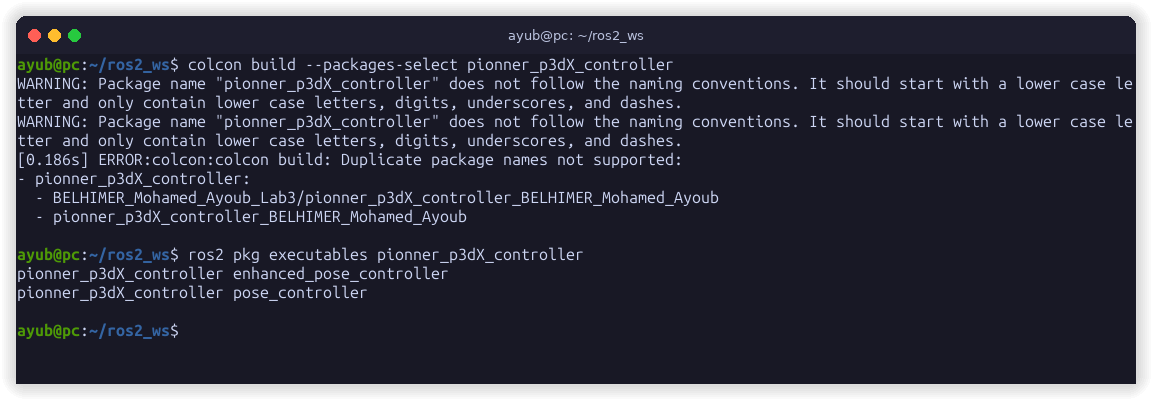
\includegraphics[width=0.92\linewidth]{colcon_build.png}
  \caption{Successful compilation of \texttt{pionner\_p3dX\_controller} via \texttt{colcon build} and verification of both registered executables (\texttt{pose\_controller} and \texttt{enhanced\_pose\_controller}).}
  \label{fig:colcon_build}
\end{figure}

\subsubsection*{Task 7: ROS 2 Bag Recording and Playback}
All active simulation topics were recorded into the MCAP bag \texttt{Lab3\_BELHIMER\_Mohamed\_Ayoub} during closed-loop execution and verified with \texttt{ros2 bag info} and \texttt{ros2 bag play}:
\begin{lstlisting}[language=bash]
$ ros2 bag record -a -o Lab3_BELHIMER_Mohamed_Ayoub
$ ros2 bag info Lab3_BELHIMER_Mohamed_Ayoub
$ ros2 bag play Lab3_BELHIMER_Mohamed_Ayoub
\end{lstlisting}
The recorded Part 1 bag spans $50.30\,\text{s}$ ($1.4\,\text{MiB}$, $1469$ total messages, including $484$ \texttt{/cmd\_vel} messages and $483$ \texttt{/pose} messages).

\subsubsection*{Task 8: PlotJuggler Visualization (Initial Controller)}
The recorded bag was loaded in PlotJuggler to inspect control inputs $(v, \omega)$, pose evolution $(x, y, \theta)$, and the 2D trajectory in the $xy$-plane.

\begin{figure}[H]
  \centering
  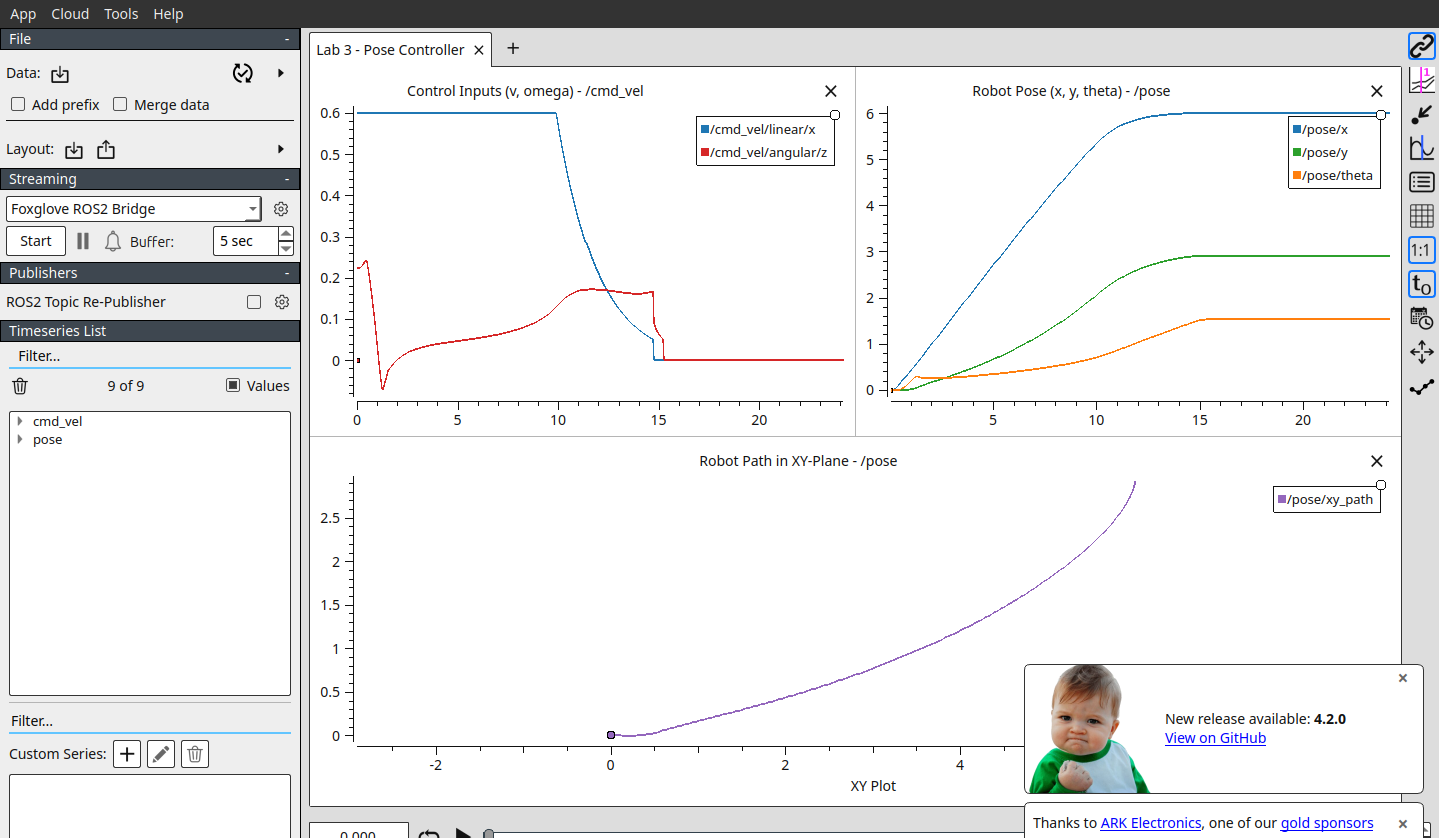
\includegraphics[width=0.95\linewidth]{plotjuggler_p1.png}
  \caption{PlotJuggler visualization of Part 1 (\texttt{pose\_controller}): \texttt{/cmd\_vel} inputs (top-left), \texttt{/pose} state signals (top-right), and 2D $xy$-path (bottom).}
  \label{fig:pj_p1}
\end{figure}

\begin{figure}[H]
  \centering
  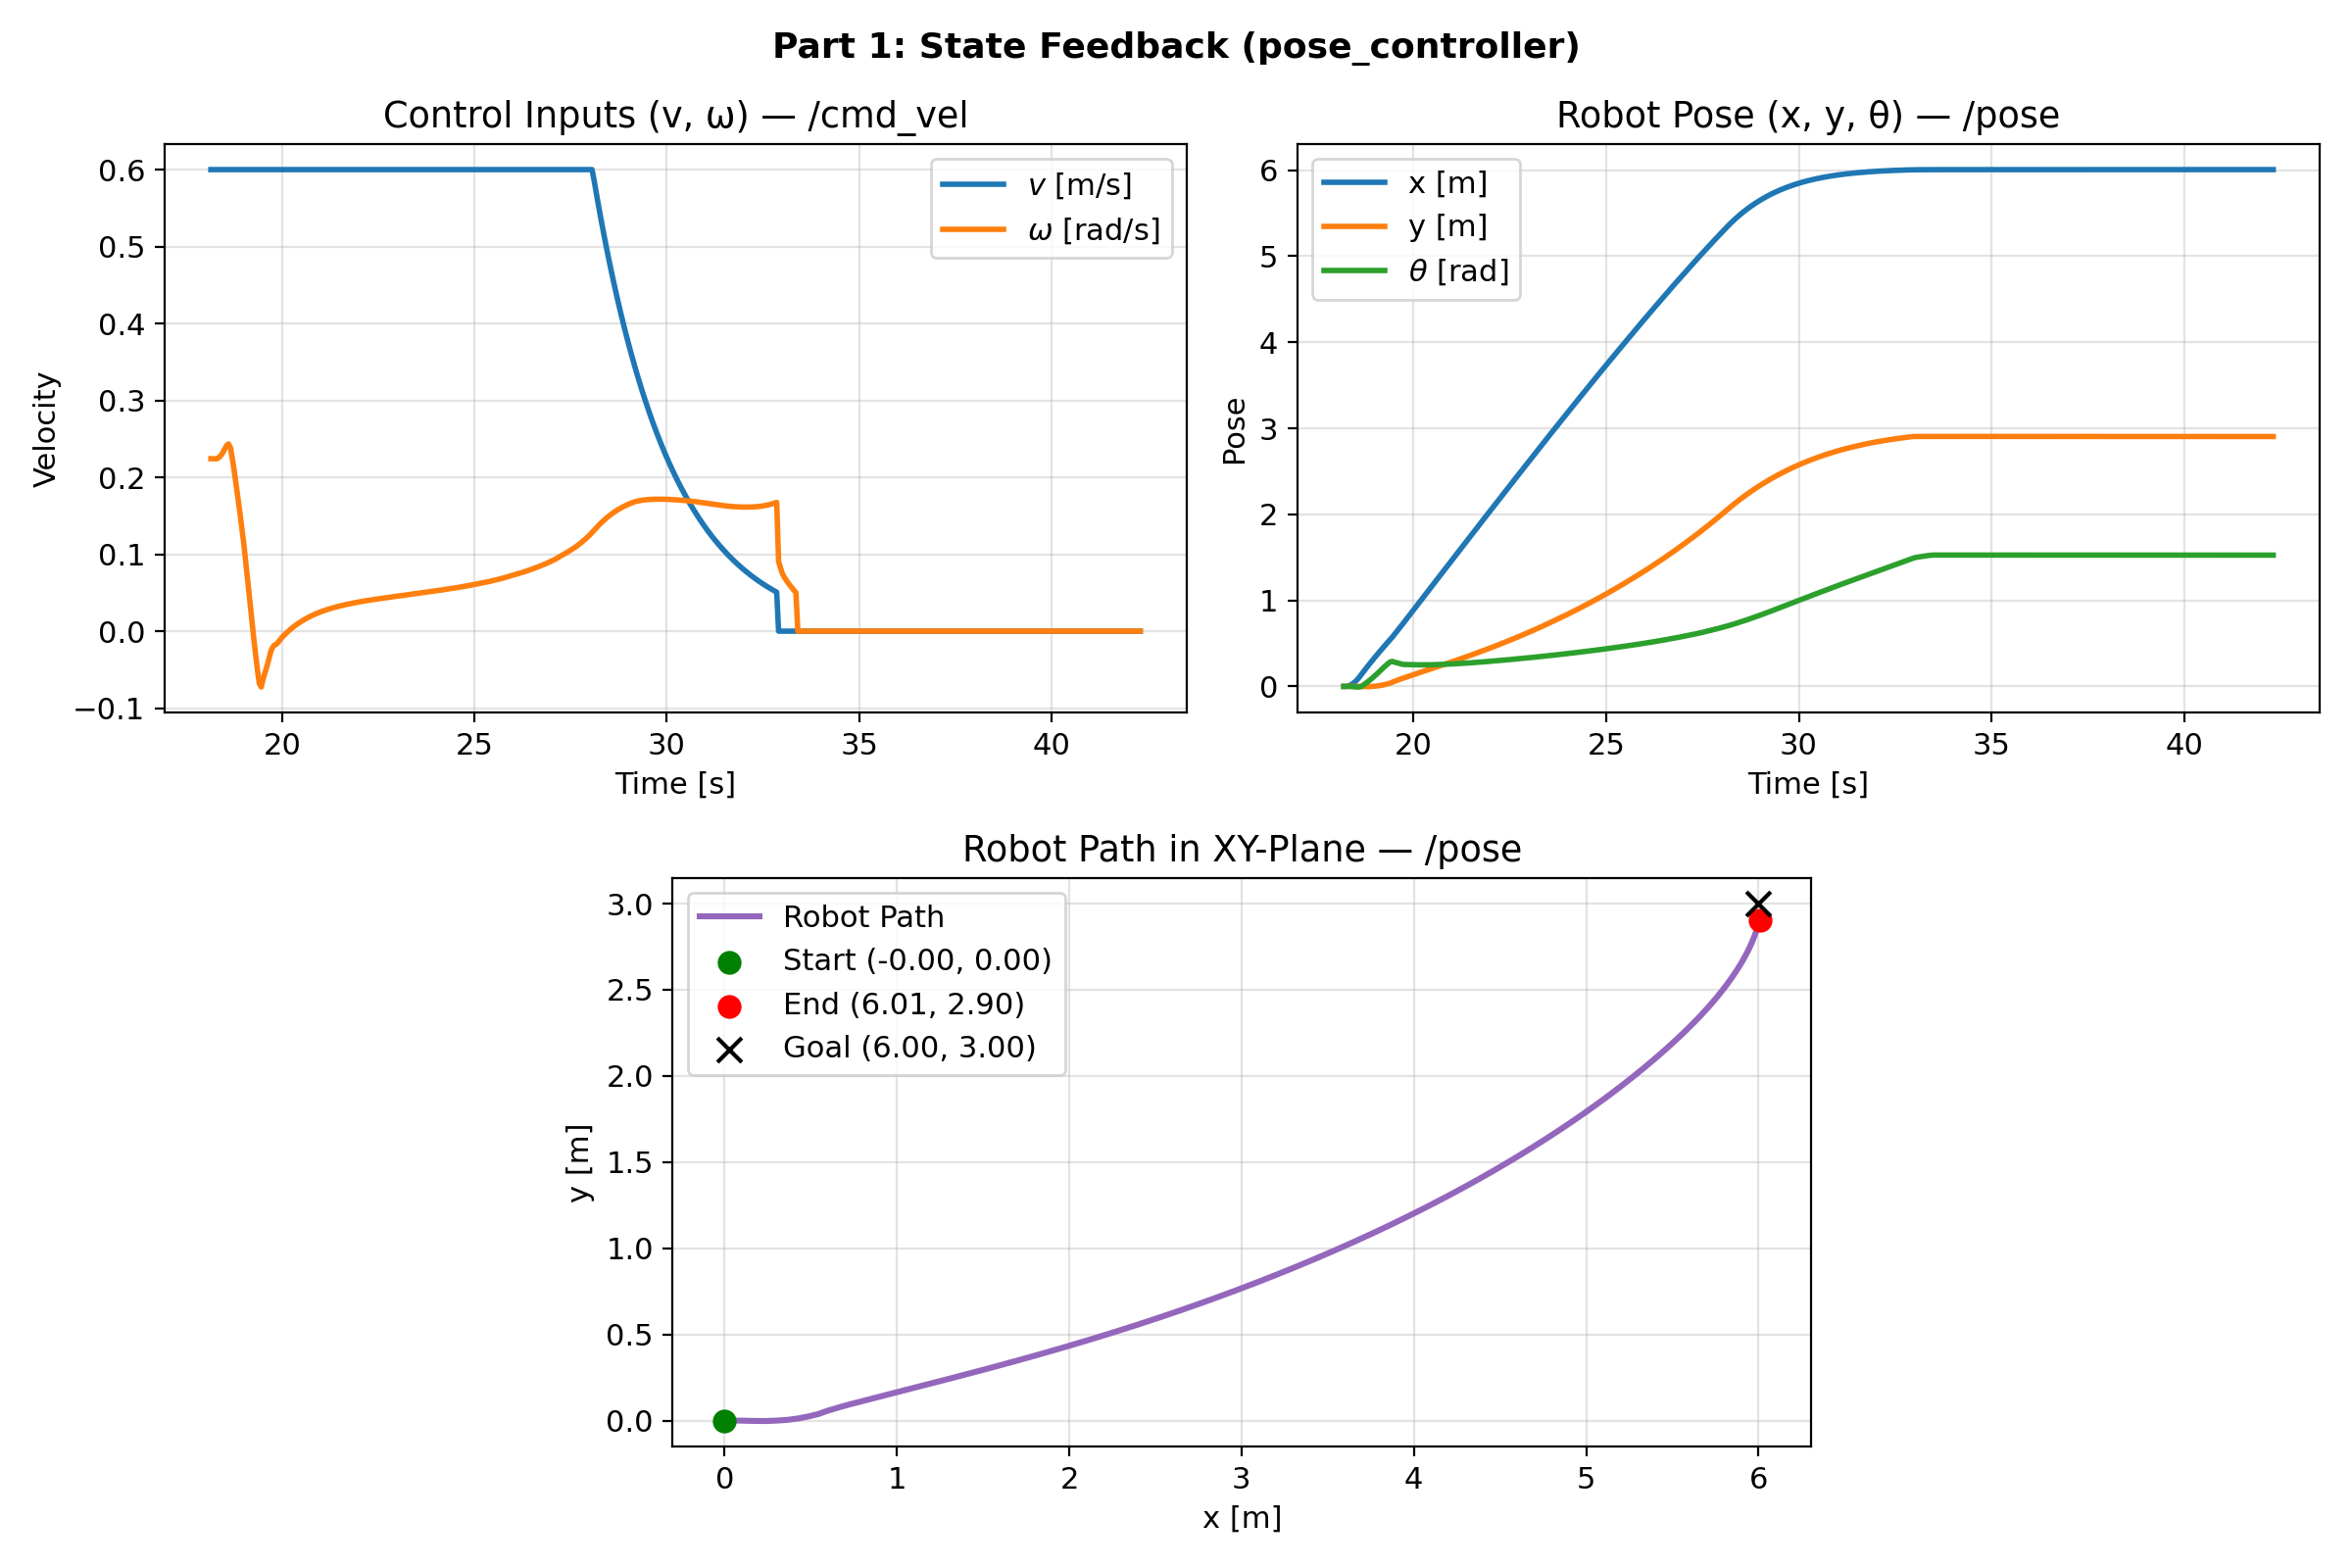
\includegraphics[width=0.92\linewidth]{p1_all_plots.png}
  \caption{High-resolution summary of Part 1 (\texttt{pose\_controller}) showing start $(-0.00, 0.00)$ to goal $(6.00, 3.00)$ convergence.}
  \label{fig:p1_plots}
\end{figure}

\subsubsection*{Task 9: Results Analysis and Conclusion (Part 1)}
\paragraph{Quantitative Results:}
\begin{itemize}
  \item \textbf{Active trajectory duration:} $15.21\,\text{s}$ ($t = 18.15\,\text{s}$ to $33.35\,\text{s}$).
  \item \textbf{Final pose (\texttt{/pose}):} $x = 6.0068\,\text{m}$, $y = 2.9043\,\text{m}$, $\theta = 1.5258\,\text{rad}$ ($87.42^\circ$).
  \item \textbf{Residual errors:} Position error $= 0.0960\,\text{m}$ ($\le 0.1\,\text{m}$), orientation error $= 0.0450\,\text{rad} = 2.58^\circ$ ($\le 0.05\,\text{rad}$).
\end{itemize}

\paragraph{Analysis:}
From $t = 18.15\,\text{s}$ to $28.0\,\text{s}$, the proportional demand $k_\rho \rho$ exceeds $v_{\max} = 0.6\,\text{m/s}$, so linear velocity saturates at $0.600\,\text{m/s}$ while $\omega$ smoothly steers the heading toward the curved approach path. Once $\rho < 1.2\,\text{m}$ ($t > 28.0\,\text{s}$), $v = 0.5\rho$ decays exponentially from $0.60\,\text{m/s}$ down to $0.051\,\text{m/s}$ before entering the position tolerance at $t \approx 32.9\,\text{s}$, followed by a brief $0.45\,\text{s}$ in-place rotation to satisfy the heading tolerance.

\paragraph{Conclusion:}
The state-feedback controller reliably drives the Pioneer P3-DX to the target pose within tolerance when the gains satisfy Equations (3)--(5). However, the exponential velocity decay ($v = k_\rho \rho$) causes noticeably slow final approach over the last meter, and the restriction $v \ge 0$ prevents reversing when goals lie behind the robot.

\newpage
% =============================================================================
% SECTION 2: STATE FEEDBACK CONTROL ENHANCED
% =============================================================================
\section{State Feedback Control Enhanced}
\subsection*{Tasks}

\subsubsection*{Tasks 1--2: \texttt{enhanced\_pose\_controller} Design and Implementation}
A new ROS 2 node named \texttt{enhanced\_pose\_controller} was created in \texttt{enhanced\_pose\_controller.py}, registered in \texttt{setup.py}, and configured in \texttt{config/pose\_controller\_params.yaml} to overcome both limitations of the initial controller:

\begin{enumerate}
  \item \textbf{Bidirectional Motion (Forward and Backward):}
  Given $\alpha = \operatorname{wrap}(\phi - \theta)$, the controller checks whether the target lies in front of or behind the robot:
  \[
    \text{if } |\alpha| > \frac{\pi}{2}: \quad
    \text{direction} = -1, \quad
    \alpha \leftarrow \operatorname{wrap}(\alpha - \pi); \qquad
    \text{else}: \quad
    \text{direction} = +1.
  \]
  In both cases, $\beta = \operatorname{wrap}(\theta_g - \theta - \alpha)$, ensuring $\alpha + \beta = \theta_g - \theta$ so convergence $(\alpha, \beta) \to (0, 0)$ always aligns $\theta \to \theta_g$. The raw linear command is then $v_{\text{raw}} = \text{direction} \cdot k_\rho \rho$, while $\omega_{\text{raw}} = k_\alpha \alpha + k_\beta \beta$ retains the exact same steering sign structure.

  \item \textbf{Constant Speed Scaling Preserving $v/\omega$:}
  To eliminate slow exponential decay near the goal without altering the path geometry, both control outputs are scaled by the same positive factor $s$:
  \[
    s = \frac{v_{\text{const}}}{|v_{\text{raw}}|}, \qquad
    v = v_{\text{raw}} \cdot s = \text{direction} \cdot v_{\text{const}}, \qquad
    \omega = \omega_{\text{raw}} \cdot s,
  \]
  with $v_{\text{const}} = 0.5\,\text{m/s}$. Whenever $|\omega| > \omega_{\max}$ ($1.2\,\text{rad/s}$), both $v$ and $\omega$ are jointly scaled by $\omega_{\max}/|\omega|$ so actuator limits are respected while keeping the curvature $\kappa = \omega/v$ invariant.
\end{enumerate}

\subsubsection*{Task 3: Bag Recording and PlotJuggler Visualization (Enhanced Controller)}
Two test scenarios were recorded with \texttt{enhanced\_pose\_controller}:
\begin{itemize}
  \item \textbf{Forward Run (\texttt{Lab3\_BELHIMER\_Mohamed\_Ayoub\_enhanced}):} Goal $(6.0, 3.0, \pi/2)$ from $(0, 0, 0)$.
  \item \textbf{Backward Run (\texttt{Lab3\_BELHIMER\_Mohamed\_Ayoub\_enhanced\_bwd}):} Rear goal $(-2.0, -1.0, 0.0)$ from $(0, 0, 0)$ to validate automatic reversing.
\end{itemize}

\begin{figure}[H]
  \centering
  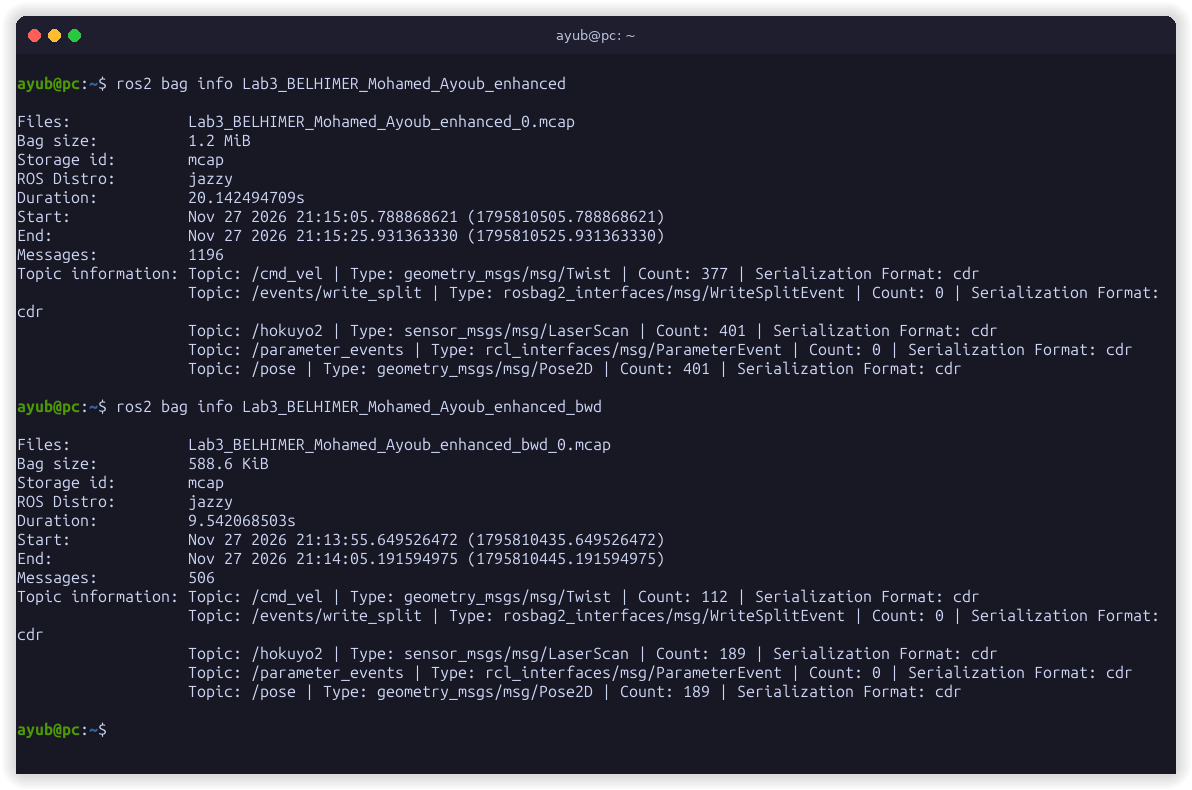
\includegraphics[width=0.92\linewidth]{ros2_bag_info.png}
  \caption{ROS 2 bag metadata inspection via \texttt{ros2 bag info} for the Part 2 forward and backward MCAP recordings.}
  \label{fig:bag_info_p2}
\end{figure}

\begin{figure}[H]
  \centering
  \begin{subfigure}[b]{0.49\linewidth}
    \centering
    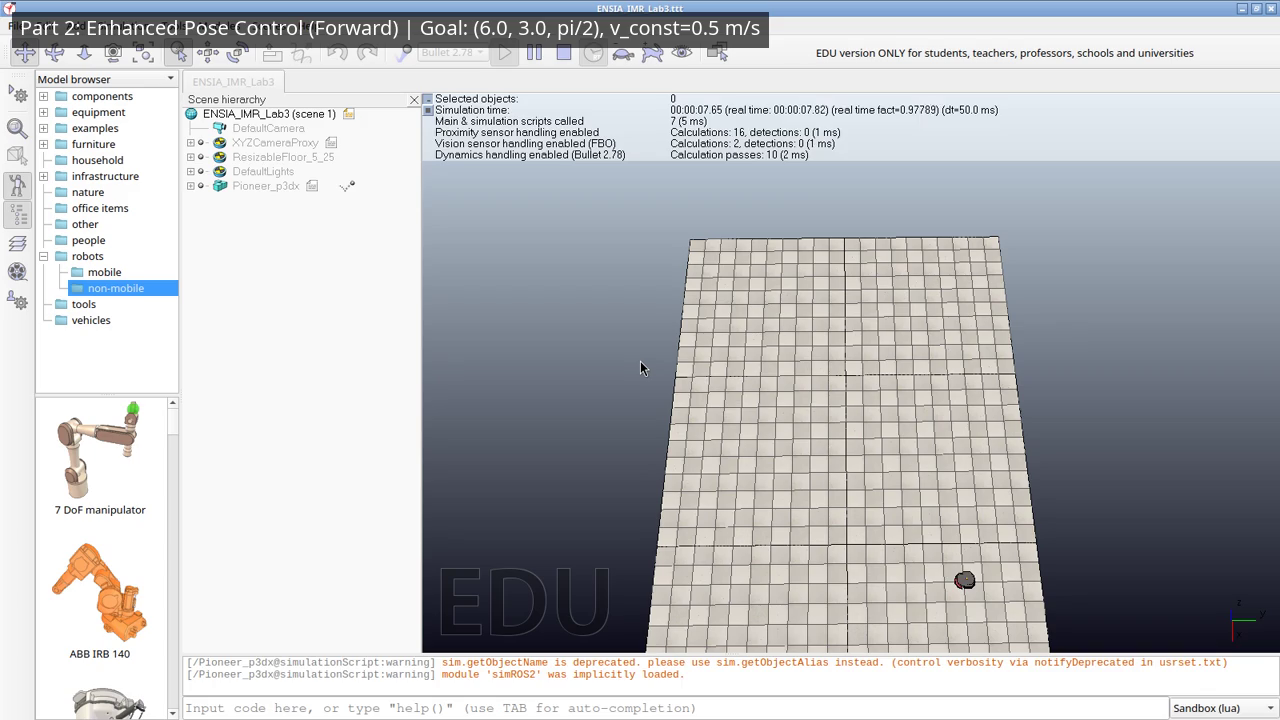
\includegraphics[width=\linewidth]{sim_p2_fwd_goal.png}
  \end{subfigure}
  \hfill
  \begin{subfigure}[b]{0.49\linewidth}
    \centering
    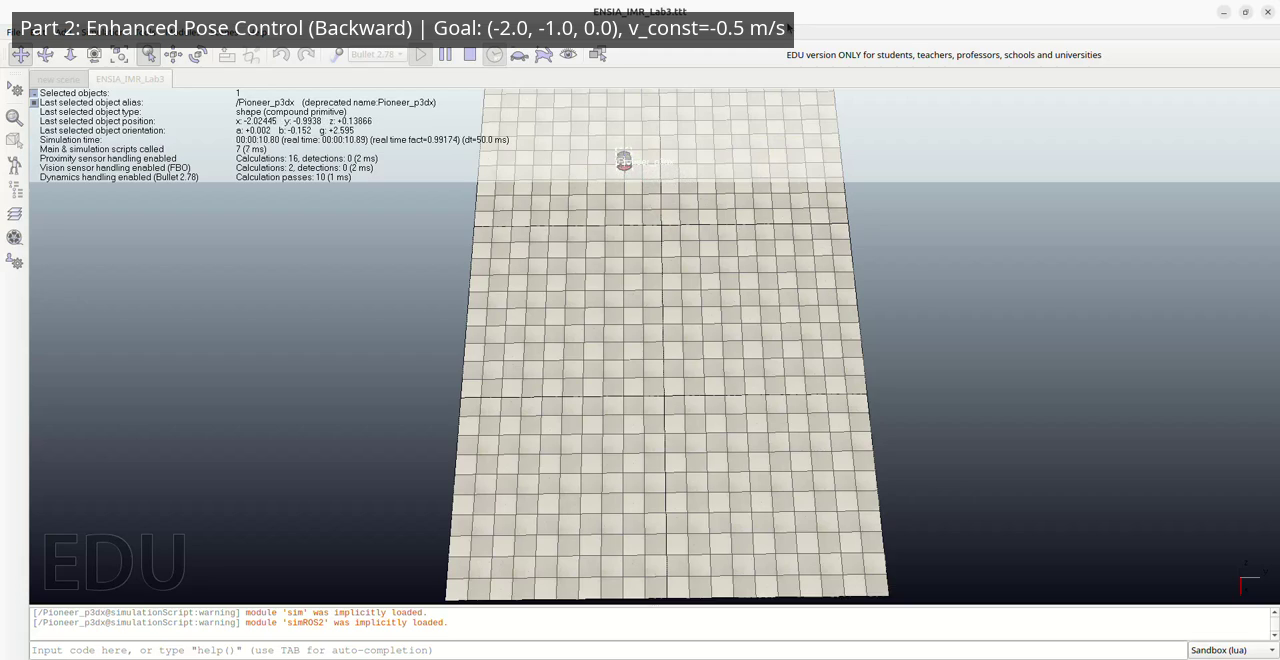
\includegraphics[width=\linewidth]{sim_p2_bwd_goal.png}
  \end{subfigure}
  \caption{CoppeliaSim final robot poses for \texttt{enhanced\_pose\_controller}: forward run at $(5.98, 3.02, 1.62)$ (left) and backward run at $(-2.02, -0.99, 0.045)$ (right).}
  \label{fig:sim_p2}
\end{figure}

\begin{figure}[H]
  \centering
  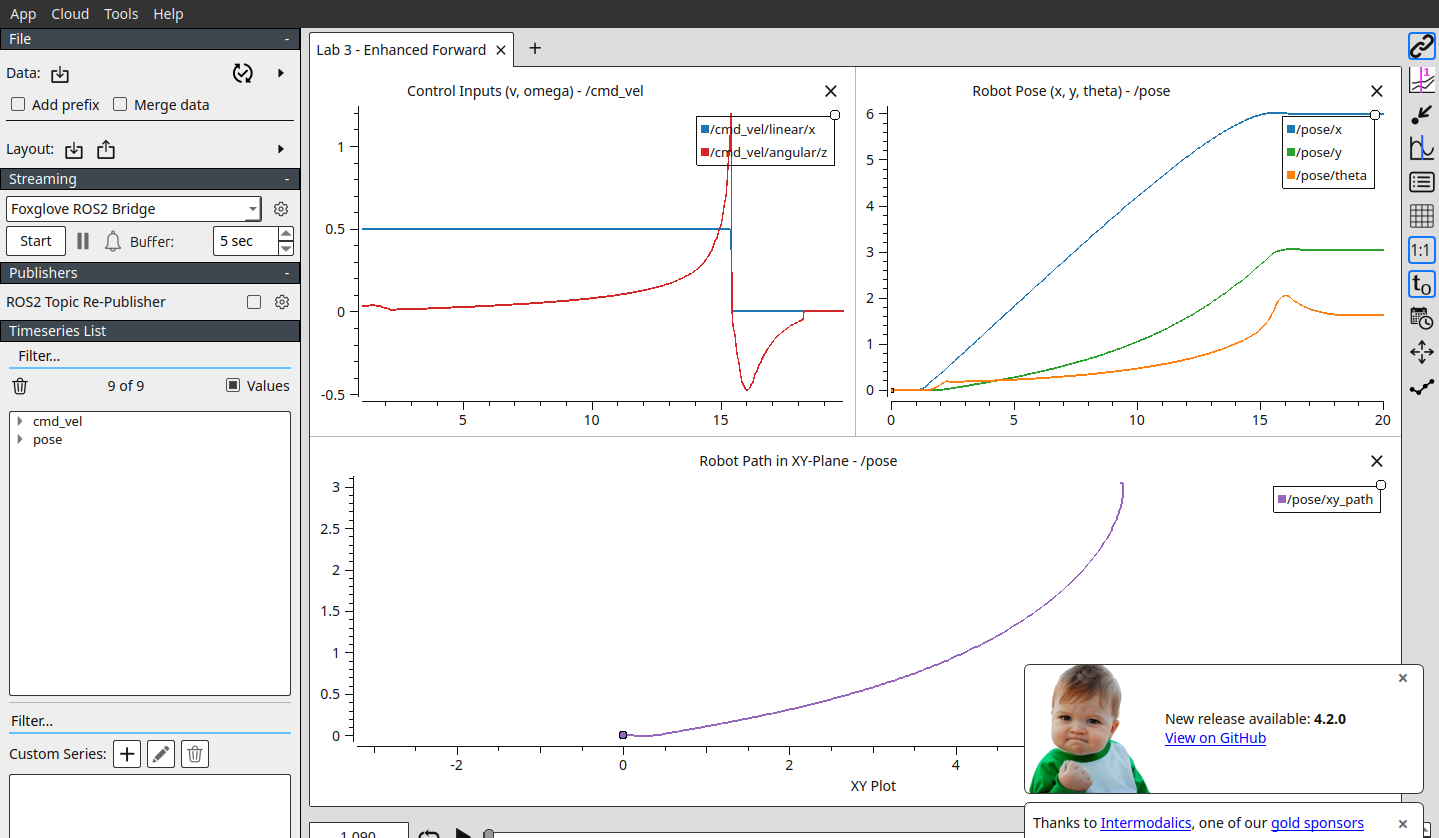
\includegraphics[width=0.95\linewidth]{plotjuggler_p2_fwd.png}
  \caption{PlotJuggler visualization of Part 2 Forward (\texttt{enhanced\_pose\_controller}): constant $v = 0.5\,\text{m/s}$ in \texttt{/cmd\_vel} (top-left), pose evolution (top-right), and $xy$-path (bottom).}
  \label{fig:pj_p2_fwd}
\end{figure}

\begin{figure}[H]
  \centering
  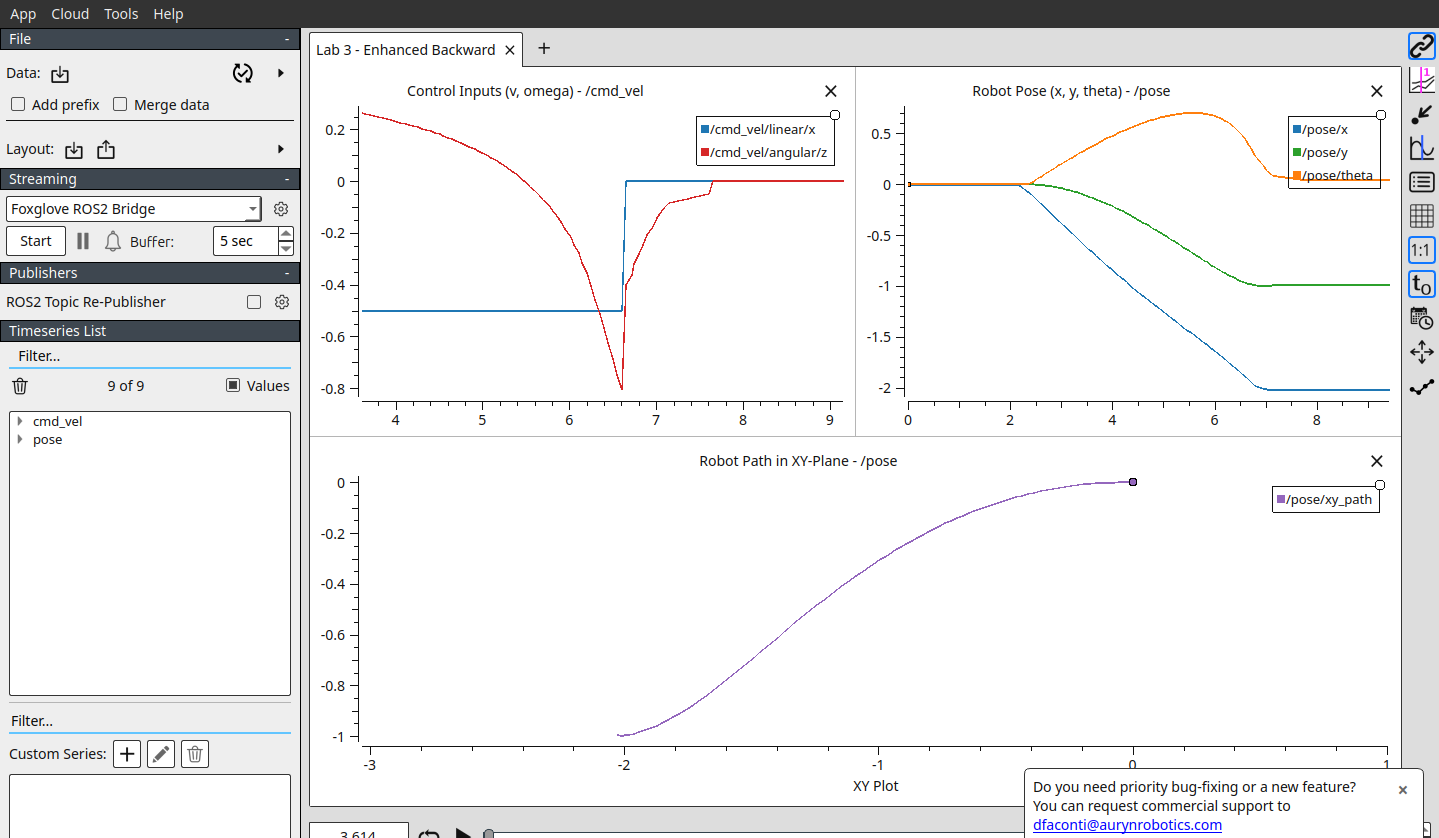
\includegraphics[width=0.95\linewidth]{plotjuggler_p2_bwd.png}
  \caption{PlotJuggler visualization of Part 2 Backward (\texttt{enhanced\_pose\_controller}): constant reverse $v = -0.5\,\text{m/s}$ in \texttt{/cmd\_vel} (top-left), pose evolution (top-right), and reverse $xy$-path to $(-2.0, -1.0)$ (bottom).}
  \label{fig:pj_p2_bwd}
\end{figure}

\begin{figure}[H]
  \centering
  \begin{subfigure}[b]{0.49\linewidth}
    \centering
    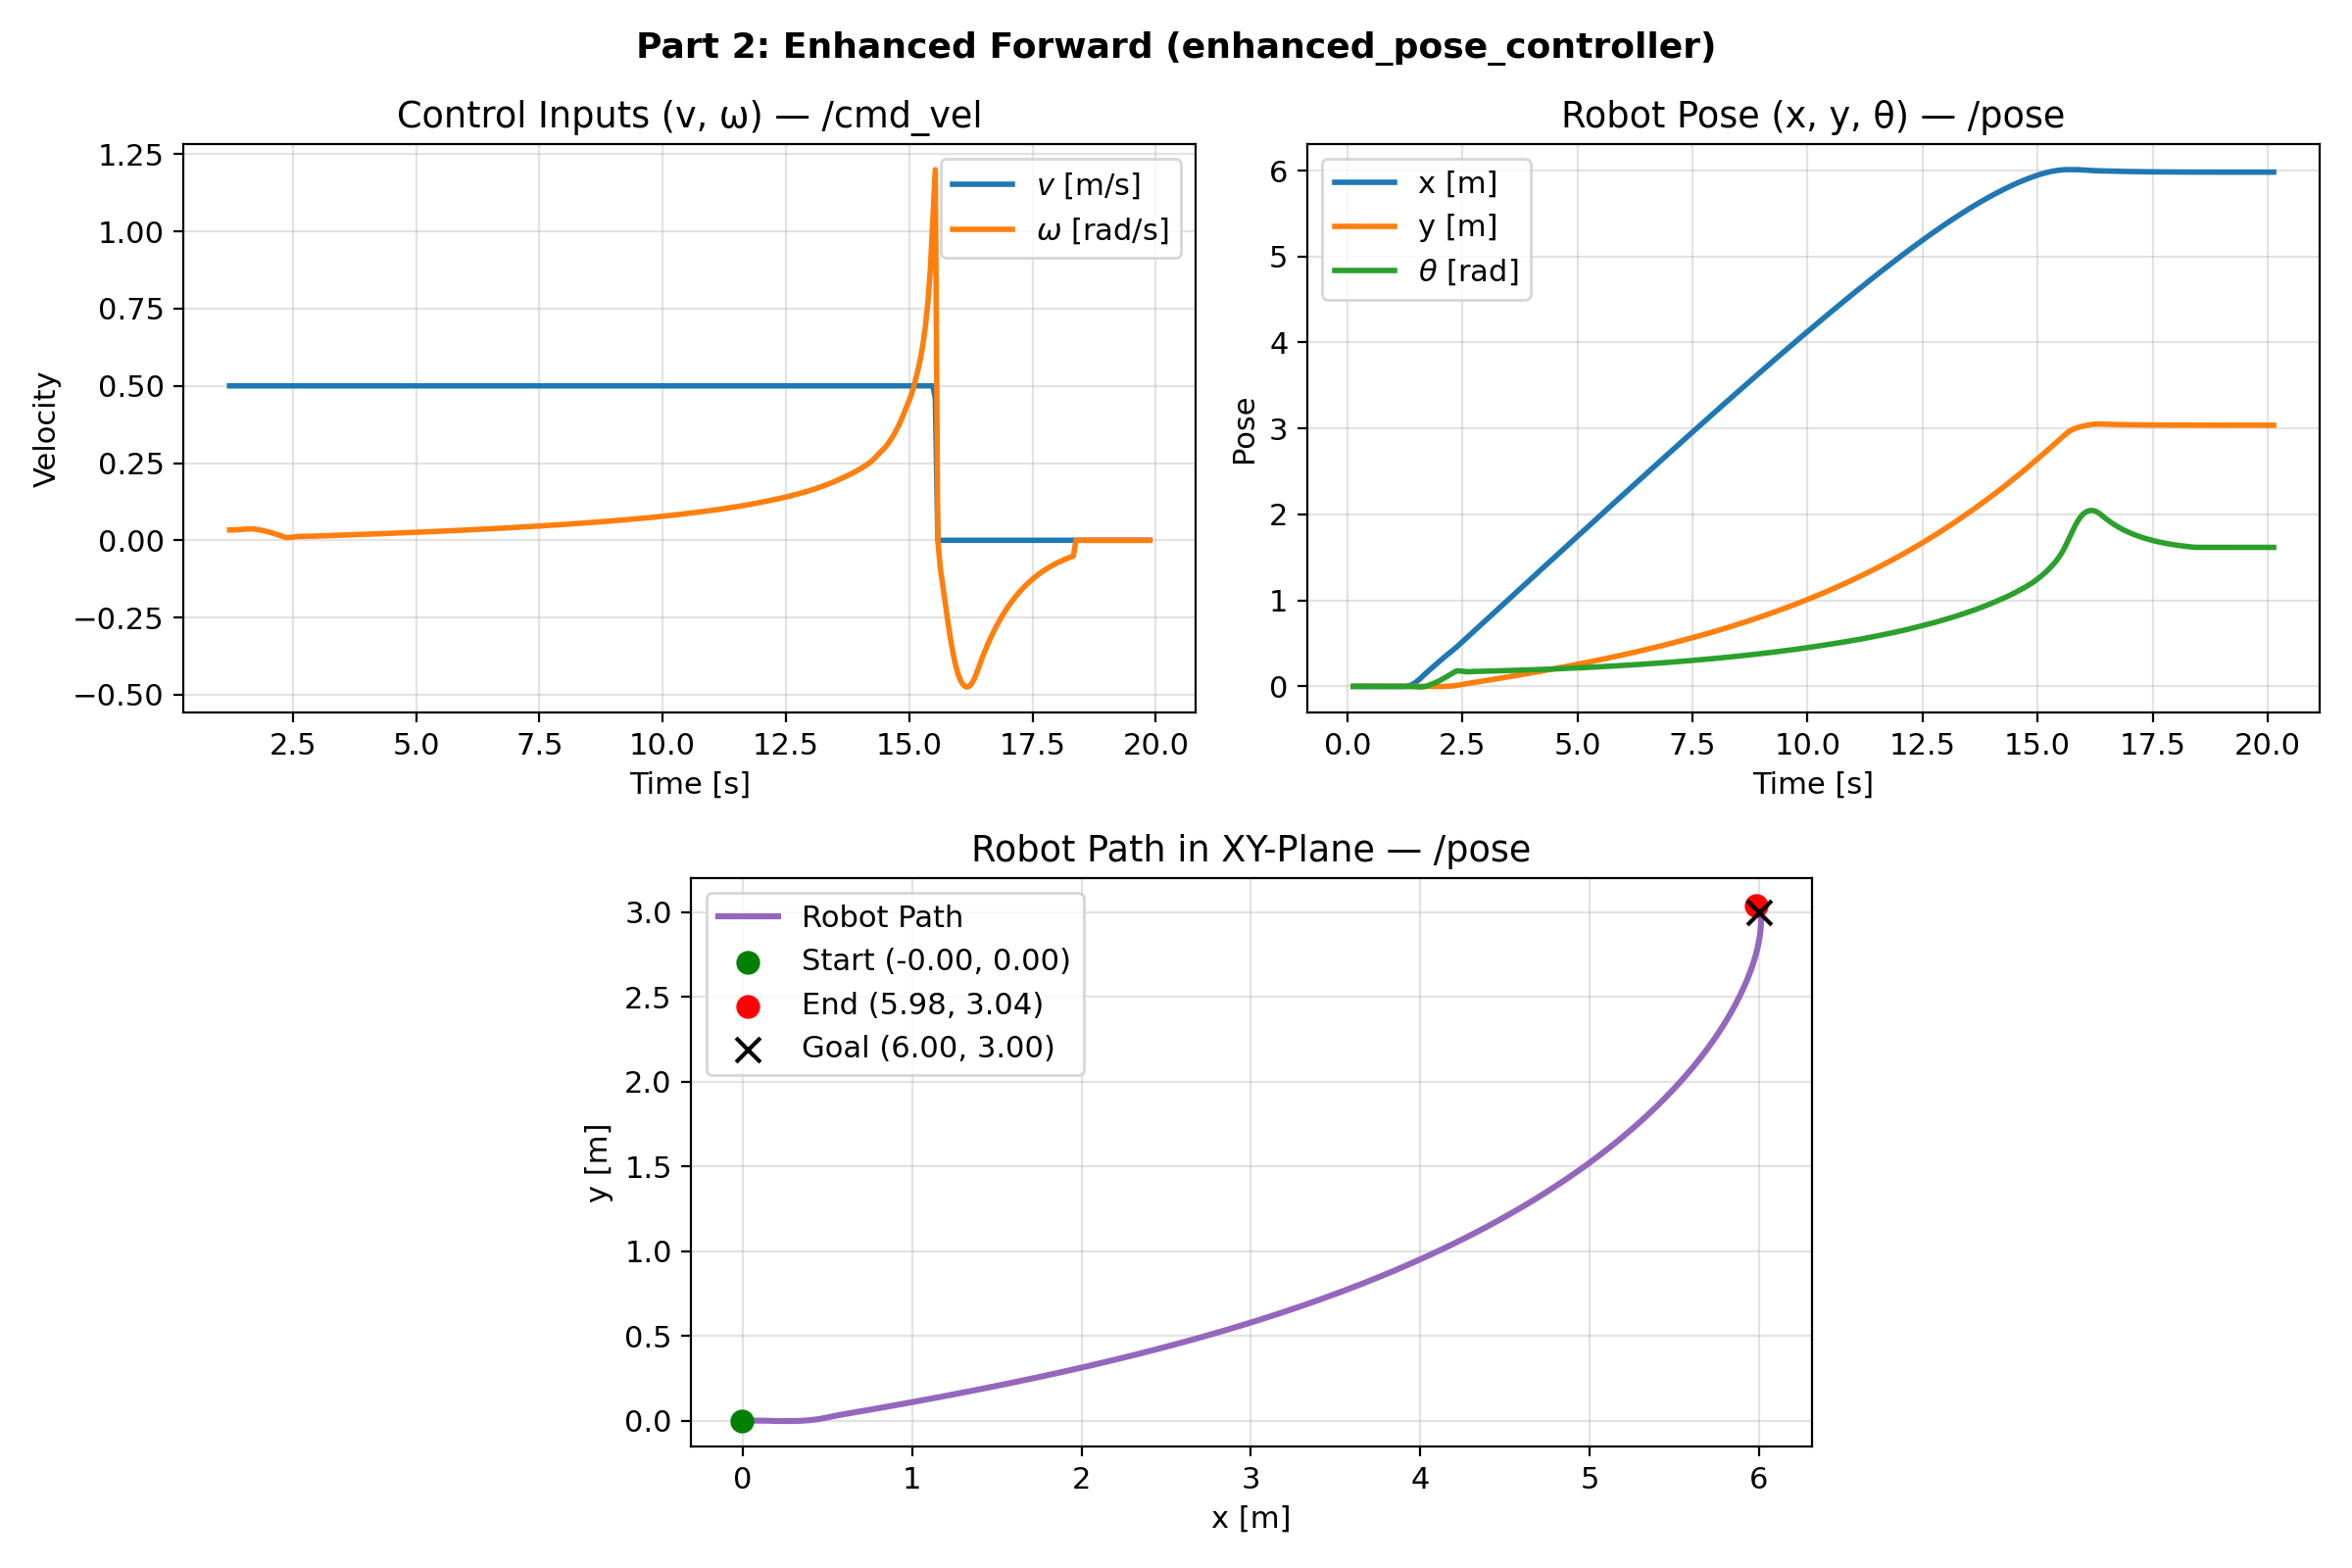
\includegraphics[width=\linewidth]{p2_fwd_all_plots.png}
  \end{subfigure}
  \hfill
  \begin{subfigure}[b]{0.49\linewidth}
    \centering
    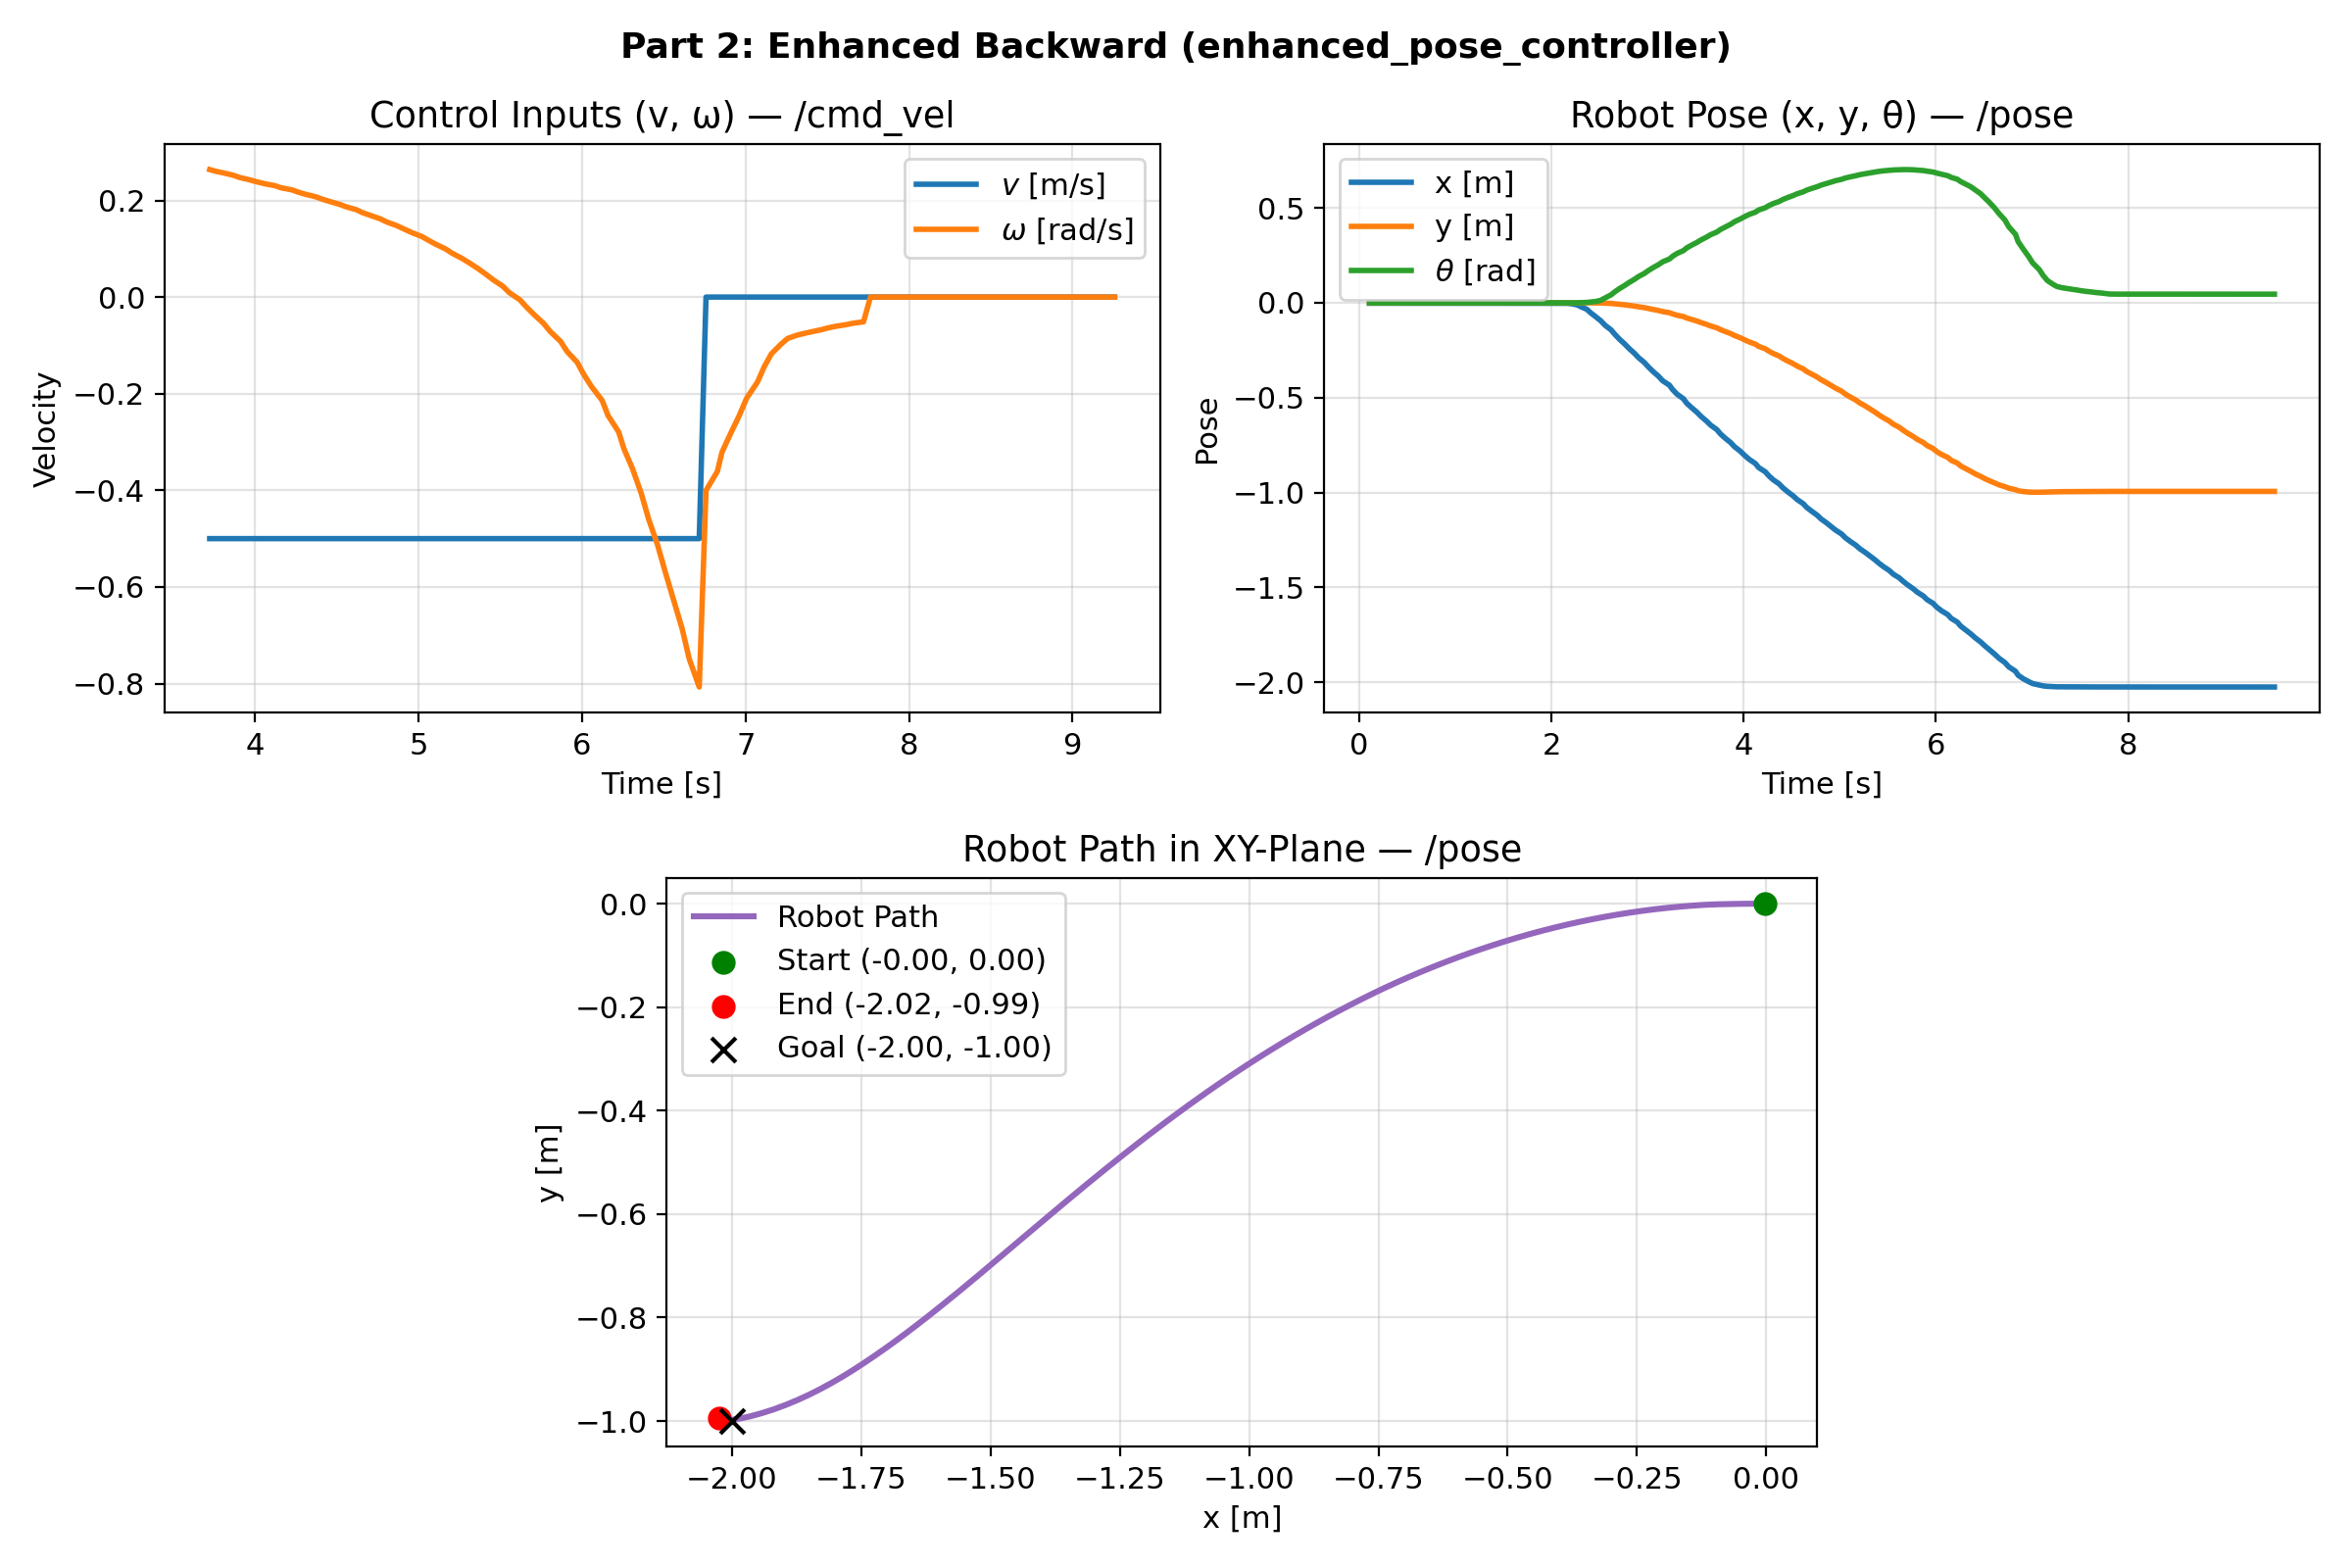
\includegraphics[width=\linewidth]{p2_bwd_all_plots.png}
  \end{subfigure}
  \caption{Detailed 3-panel summaries for \texttt{enhanced\_pose\_controller}: forward run to $(6.0, 3.0, \pi/2)$ (left) and backward run to $(-2.0, -1.0, 0.0)$ (right).}
  \label{fig:p2_summaries}
\end{figure}

\begin{figure}[H]
  \centering
  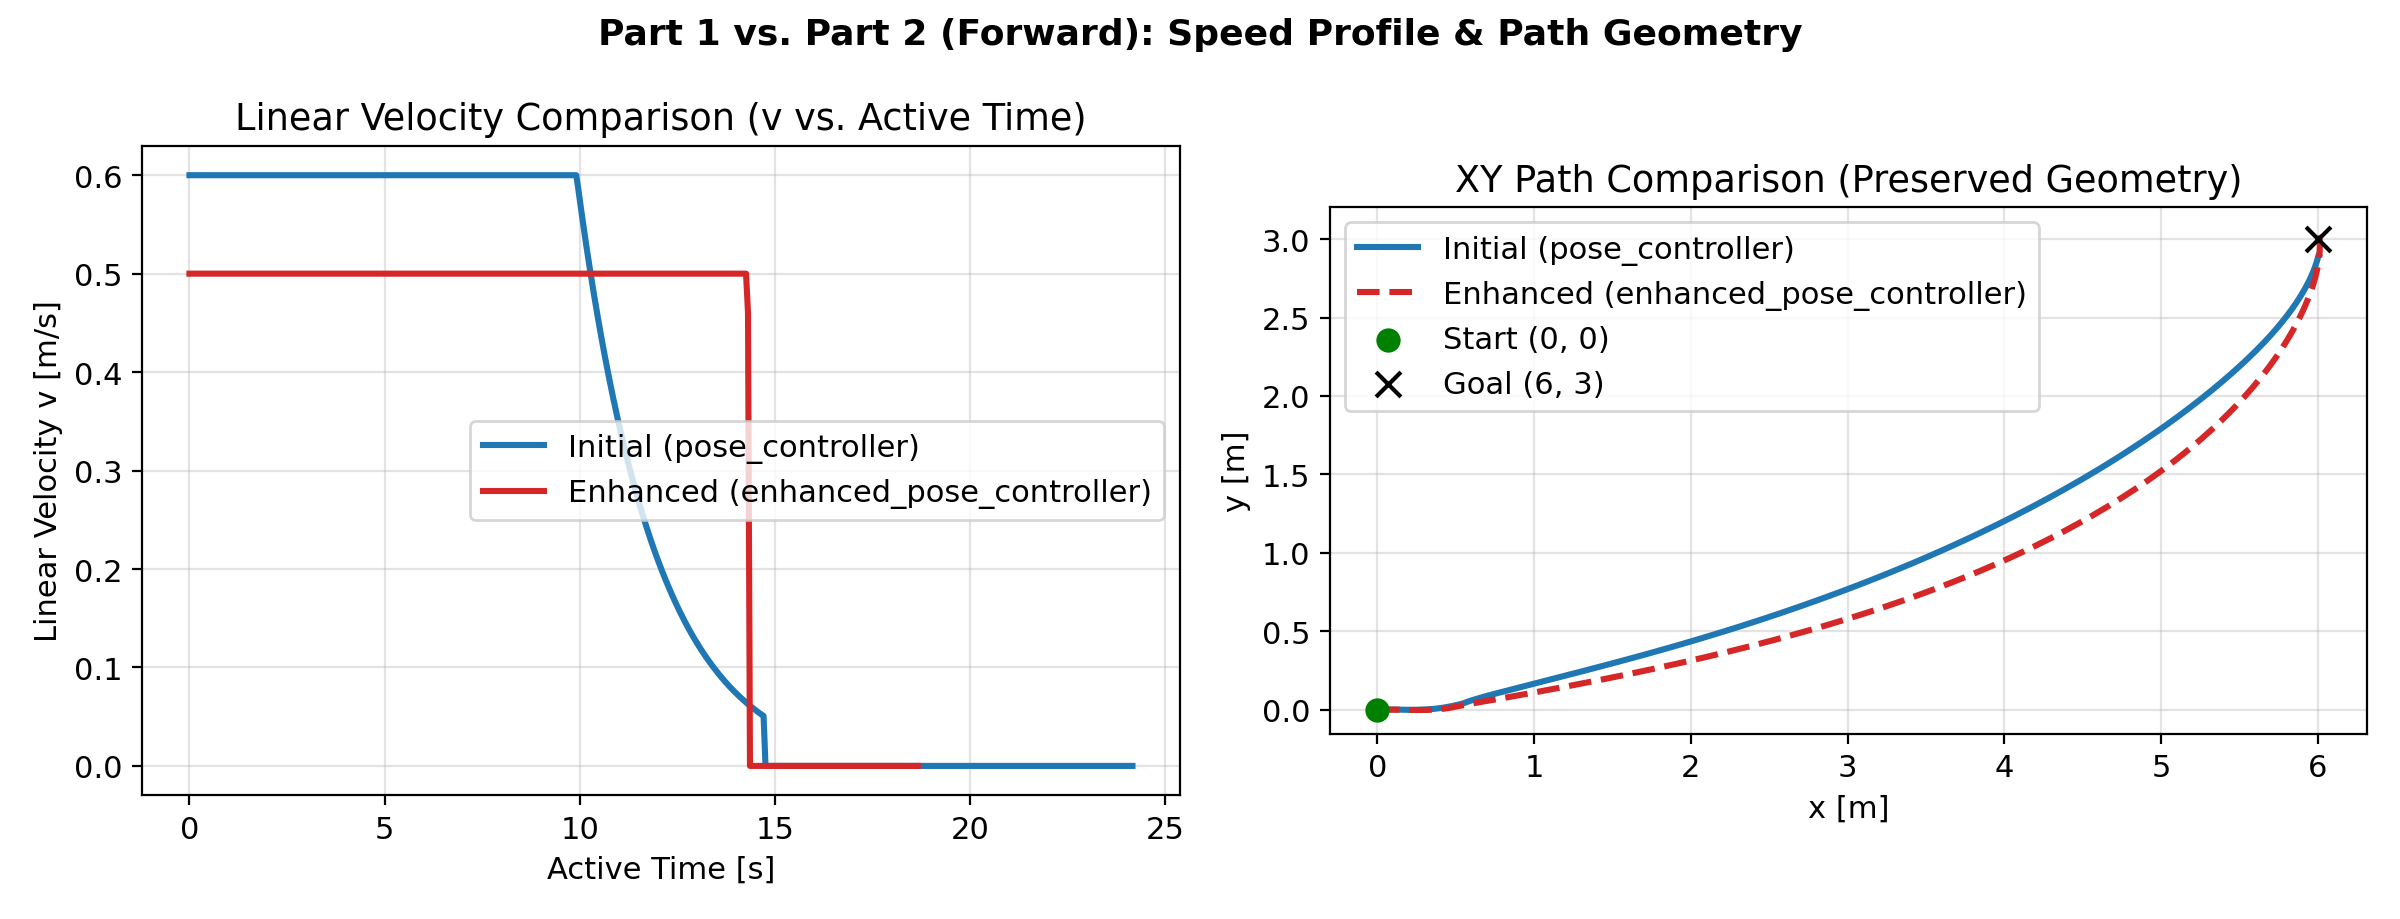
\includegraphics[width=0.95\linewidth]{comparison_p1_vs_p2.png}
  \caption{Direct comparison between initial (\texttt{pose\_controller}) and enhanced (\texttt{enhanced\_pose\_controller}) forward trajectories: linear velocity profiles (left) and $xy$-paths (right).}
  \label{fig:p1_vs_p2}
\end{figure}

\subsubsection*{Task 4: Comparative Analysis and Conclusion (Part 2)}
Table~\ref{tab:comparison} summarizes the measured performance across all three recorded experiments.

\begin{table}[H]
  \centering
  \small
  \caption{Quantitative performance comparison between initial and enhanced controllers.}
  \label{tab:comparison}
  \resizebox{\linewidth}{!}{%
  \begin{tabular}{lccccc}
    \toprule
    \textbf{Controller / Scenario} & \textbf{Goal $(x_g, y_g, \theta_g)$} & \textbf{Active Time} & \textbf{Linear Vel. $v$} & \textbf{Pos. Error} & \textbf{Ori. Error} \\
    \midrule
    Initial (\texttt{pose\_controller}) & $(6.0,\, 3.0,\, \pi/2)$ & $15.21\,\text{s}$ & $[0.051,\, 0.600]\,\text{m/s}$ & $0.0960\,\text{m}$ & $2.58^\circ$ \\
    Enhanced (Forward) & $(6.0,\, 3.0,\, \pi/2)$ & $17.11\,\text{s}$ & $+0.500\,\text{m/s}$ (const) & $0.0415\,\text{m}$ & $2.61^\circ$ \\
    Enhanced (Backward) & $(-2.0,\, -1.0,\, 0.0)$ & $4.00\,\text{s}$ & $-0.500\,\text{m/s}$ (const) & $0.0252\,\text{m}$ & $2.60^\circ$ \\
    \bottomrule
  \end{tabular}}
\end{table}

\paragraph{Analysis of Results:}
\begin{itemize}
  \item \textbf{Constant-Speed Convergence:} In the enhanced forward run, $v$ stays strictly constant at $+0.500\,\text{m/s}$ throughout Phase~1, reaching the target position in $14.3\,\text{s}$ (even faster than the initial controller's $14.7\,\text{s}$ despite having a lower peak speed of $0.5\,\text{m/s}$ vs.\ $0.6\,\text{m/s}$). Because $s = v_{\text{const}}/(k_\rho \rho)$ grows large as $\rho \to 0.1\,\text{m}$, $\omega$ peaks briefly at $\omega_{\max} = 1.20\,\text{rad/s}$ just before entering the distance tolerance, producing a slight heading overshoot ($\approx 2.0\,\text{rad}$) that Phase~2 smoothly corrects back to $1.616\,\text{rad}$ over the final $2.8\,\text{s}$.
  \item \textbf{Path Geometry ($v/\omega$ Invariance):} In Figure~\ref{fig:p1_vs_p2} (right), the enhanced controller follows a slightly tighter curve than the initial controller. This occurs because the initial controller saturated $v$ alone at $v_{\max} = 0.6\,\text{m/s}$ during the first $10\,\text{s}$ without scaling $\omega$, altering the $v/\omega$ ratio, whereas the enhanced controller scales $(v, \omega)$ jointly and preserves the true un-saturated state-feedback trajectory.
  \item \textbf{Bidirectional Maneuverability:} For the rear goal $(-2.0, -1.0, 0.0)$, $|\alpha| = 2.68\,\text{rad} > \pi/2$, so \texttt{enhanced\_pose\_controller} immediately selects $v = -0.500\,\text{m/s}$ and reaches the goal in just $4.00\,\text{s}$ with $0.0252\,\text{m}$ position error and $2.60^\circ$ orientation error---completely avoiding an inefficient $180^\circ$ turnaround.
\end{itemize}

\paragraph{Overall Conclusion:}
The enhanced state-feedback pose controller successfully addresses both practical shortcomings of the baseline formulation. By scaling $(v, \omega)$ proportionally to maintain a constant cruising speed while preserving the curvature ratio $v/\omega$, it eliminates slow asymptotic crawling near the target. Furthermore, incorporating the $|\alpha| > \pi/2$ direction switch enables natural forward and backward motion, yielding shorter, smoother, and time-efficient trajectories across arbitrary goal poses.

\end{document}
